\chapter[EMERGENCY]{EMERGENCY PROCEDURES}
\thumbtab{Em Proc}{1}
\localtableofcontents
\thispagestyle{plain}
\cleardoublepage

\section{TAKEOFF --- WIP}

\begin{center}
    \vspace{4em}%
    \Large\titlefont%
    \textbf{COMING SOON}%
\end{center}

\clearpage

\marginfigeometry

\section{IN-FLIGHT}

\subsection{AIRSTART}

\begin{checklistenumerate}
    \blueitem[Throttle]\dotfill \textbf{OFF}, then \textbf{midrange}
    \marnotebox{\small
        If at low altitude, initiate a zoom climb and jettison stores (if required)
    }
    \begin{itemize}
        \item monitor for signs of light-off
        \item if RPM \& FTIT continue decay with RPM below 50\%, continue procedure
    \end{itemize}
    \blueitem[ENG CONT Switch]\dotfill \textbf{SEC}
    \begin{itemize}
        \item even if SEC caution light is illuminated
    \end{itemize}
    \blueitem[Airspeed] 
    --- attain approximately 250 kts 
    \marnotebox{\small
        Above 30'000 ft MSL airspeeds in 
        250-400 kts / 0.9 mach range increase probability of successful airstart

        \bigskip
        If glide range not a factor, consider maintaining 250 kts above 10'000 ft AGL
    }

    \medskip
    With JFS RUN light on can reduce airspeed
    \begin{itemize}
        \item maximum range --- 200 kts
        \item maximum endurance --- 170 kts
        \item plus 5 kts per 1000 lbs of fuel / stores 
    \end{itemize}
    \blueitem[JFS Switch]\dotfill \textbf{START 2}\\
    \hfill below 20'000 ft MSL and 400 kts
    \blueitem[STORES]\dotfill \textbf{Jettison}\\
    \hfill (if required)
\end{checklistenumerate}

\textbf{If RPM rolls back or hangs below in-flight idle (approx 70\%)
and FTIT exceeds 935$^\circ$C}

\begin{checklistenumerate}[resume]
    \blueitem[Throttle]\dotfill \textbf{OFF},\\
    allow FTIT to drop below 700$^\circ$C, 
    befre advancing throttle to midrange
    \blueitem[Airspeed] --- increase to 400 kts / 0.9 mach maximum
\end{checklistenumerate}

\textbf{If hung / hot start persists}

\begin{checklistenumerate}[resume]
    \blueitem[Throttle]\dotfill \textbf{OFF}
    \blueitem[ENG CONT Switch]\dotfill \textbf{SEC} if in \textbf{PRI}\\
    \hfill \textbf{PRI} if in \textbf{SEC}
    \blueitem[Throttle]\dotfill \textbf{Midrange}
\end{checklistenumerate}

\clearpage

\textbf{If engine does not respond normally after airstart is completed}

\begin{checklistenumerate}[resume]
    \blueitem[ENG CONT Switch]\dotfill \textbf{SEC}
    \blueitem[Airspeed] --- 250 kts if thrust too low to sustain level flight
    \blueitem[Throttle] --- Verify engine responds to throttle movement, set as desired
\end{checklistenumerate}

\textbf{%
    If engine does not respond normally after airstart is completed in SEC, 
    or thrust still insufficient to make safe landing
}

\begin{checklistenumerate}[resume]
    \blueitem[ENG CONT Switch]\dotfill \textbf{PRI}
    \blueitem[Refer to Flameout Landing] --- \Cref{subsec:proc_em:landing:flameout}
\end{checklistenumerate}

\textbf{If engine responds normally}

\begin{checklistenumerate}[resume]
    \blueitem[JFS Switch]\dotfill \textbf{OFF}
    \blueitem[ELEC CAUTION RESET Button]\dotfill \textbf{Press}\\
    Verify
    \begin{itemize}
        \item \textbf{MAIN GEN Light} --- \textbf{OFF}
        \item \textbf{STBY GEN Light} --- \textbf{OFF}
    \end{itemize}
    \blueitem[EPU Switch]\dotfill \textbf{OFF}\\
    \hfill then \textbf{NORM}
    \blueitem[ADI] --- check for \textbf{OFF} / \textbf{AUX} flags,
    indicates total INS failure
    \blueitem[Land as soon as possible]
\end{checklistenumerate}

\marginfigrestore

\clearpage

\section{LANDING}

\subsection{FLAMEOUT LANDING}
\label{subsec:proc_em:landing:flameout}

\notebox{
    If you are reading this section for the first time following an in-flight engine flameout, 
    eject now.
}

\paragraph{Optimal Airspeed}
\begin{itemize}
    \item \textbf{LG Up} --- 200 kts
    \item \textbf{LG Down} --- 190 kts
\end{itemize}

Increase by 5 kts for every 1000 lbs of fuel / stores

\paragraph{Optimal AOA}
\begin{itemize}
    \item \textbf{LG Up} --- 7 deg AOA achieves optimal airspeed
\end{itemize}

\paragraph{Glideslope} 
Maximum range glideslope
approx. 7nm per 5000 ft AGL with gear up,
7 deg AOA, no stores retained

\paragraph{Bank Angle}
To minimize altitude loss in turns bank at

\begin{itemize}
    \item \textbf{LG Up} --- 50 deg
    \item \textbf{LG Down} --- 55 deg  
\end{itemize}

\subsubsection{OVERHEAD APPROACH}

\paragraph{Approach Pattern}
Reference \cref{fig:proc_em:landing:flameout:overhead}, 
if overhead pattern key positions cannot be reached use a straight-in 
described in \cref{subsec:proc_em:landing:flameout:straightin}

\paragraph{A \quad High Key}
\begin{itemize}
    \item \textbf{Location} --- approx {1/3 down down the runway} from desired touchdown point
    \item \textbf{Altitude} --- {7'000-10'000 ft AGL},
    recommend 7'000 ft plus 500 ft for every 1'000 lbs of fuel/stores
\end{itemize}

\paragraph{B \quad Low Key}
\begin{itemize}
    \item \textbf{Location} --- {1 nm abeam} point of rollout for final 
    \item \textbf{Altitude} --- {3'000-5'000 ft AGL},
    recommend 3'000 ft plus 250 ft for every 1'000 lbs of fuel/stores
\end{itemize}

\paragraph{C \quad Base Key}
\begin{itemize}
    \item \textbf{Location} --- midpoint of final turn from downwind to final,
    1.25 nm from touchdown point
    \item \textbf{Altitude} --- {2'000 ft AGL minimum}
\end{itemize}

\notebox{
    \begin{itemize}
        \item EPU consumes approx 15\% EPU fuel per minute
        \item JFS reduces EPU load, conserving fuel
    \end{itemize}
}

\begin{figure}[htbp]
    \centering
    \begin{subfigure}[t]{\linewidth}
        \centering
        \begin{tikzpicture}[figstyle]

            % coordinates
            \coordinate (td_des) at (0,0);
            \coordinate (high_key) at (15,40);
            \coordinate (inter_high_low) at (30,35);
            \coordinate (low_key) at (-15,20);
            \coordinate (base_key) at (-30,12);
            \coordinate (final) at (170:15);
    
            % runway
            \fill[]
            ($(td_des)+(-5,0)$) 
            -- ($(td_des)+(45,0)$)
            -- ($(td_des)+(45,-0.5)$)
            -- ($(td_des)+(-5,-0.5)$)
            -- cycle;

            \foreach \n in {5, 10, 15, 20, 25} {
                \draw[thin]
                (\n,0) 
                -- ++(90:0.5)
                -- ++(0:3)
                -- ++(-90:0.5)
                -- cycle
                (\n+0.25,0) -- ++(90:0.5)
                (\n+2.75,0) -- ++(90:0.5);
            }

            \draw[thin]
            (9,0)
            -- ++(180:0.1)
            -- ++(90:1)
            -- ++(180:0.25)
            -- ++(90:0.25)
            -- ++(0:0.3)
            -- ++(90:0.5)
            -- ++(-90:0.5)
            -- ++(0:0.3)
            -- ++(-90:0.25)
            -- ++(180:0.25)
            -- ++(-90:1)
            -- cycle;
            
            % fighter
            \node[anchor=east] (fighter) at (high_key.west) {
                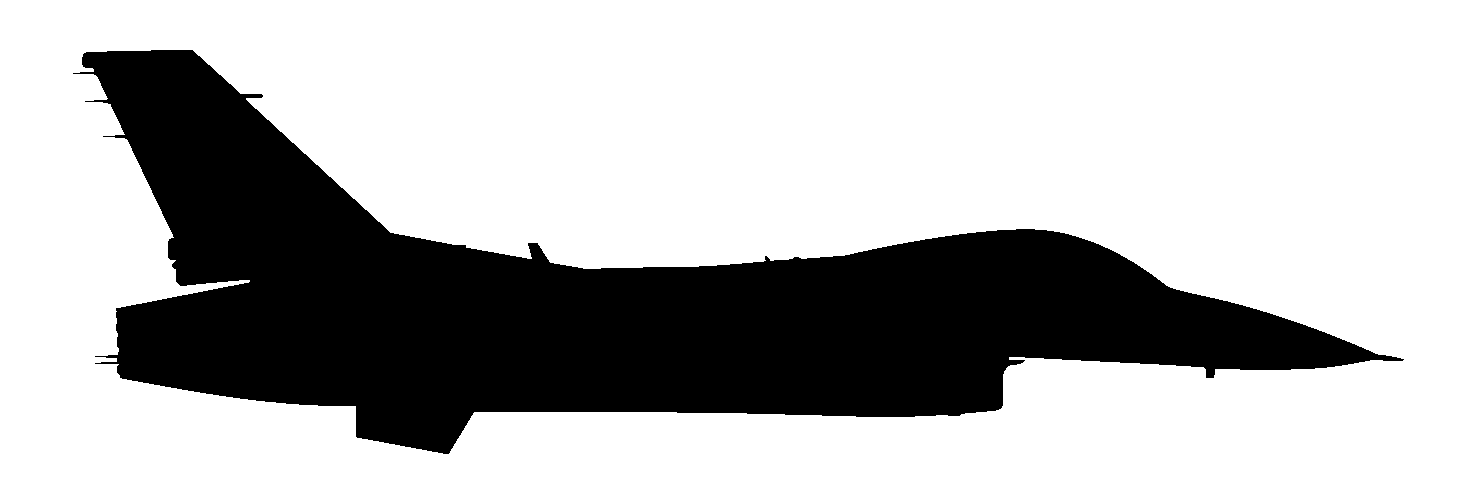
\includegraphics[
                    width=7.5mm,
                ]{diagrams/aircraft/silhouette_f16_side.pdf}
            };
    
            % approach
            \draw[->]
            (high_key)
            .. controls ($(high_key)+(0:6)$) and ($(inter_high_low)+(90:4)$) ..
            (inter_high_low)
            .. controls ($(inter_high_low)+(-90:6)$) and ($(low_key)+(10:20)$) ..
            (low_key);
            \draw[-]
            (low_key)
            .. controls ($(low_key)+(190:10)$) and ($(base_key)+(90:2)$) ..
            (base_key);
            \draw[->]
            (base_key)
            .. controls ($(base_key)+(-90:6)$) and ($(final)+(170:5)$) ..
            (final) -- (td_des);

            \node[red, font=\small\bfseries, above] at (high_key) {A};
            \node[red, font=\small\bfseries, above] at (low_key) {B};
            \node[red, font=\small\bfseries, left] at (base_key) {C};
            \node[red, font=\small\bfseries, below] at (td_des) {D};
    
            \filldraw[red] (high_key) circle (2pt);
            \filldraw[red] (low_key) circle (2pt);
            \filldraw[red] (base_key) circle (2pt);
            \filldraw[red] (td_des) circle (2pt);
        \end{tikzpicture}
        \caption{side view}
    \end{subfigure}

    \vspace{2em}
    \begin{subfigure}[t]{\linewidth}
        \centering
        \begin{tikzpicture}[figstyle]

            % coordinates
            \coordinate (td_des) at (0,0);
            \coordinate (high_key) at (15,0);

            % runway
            \draw[thick]
            ($(td_des)+(-5,-2)$) 
            -- ($(td_des)+(-5,2)$) 
            -- ($(td_des)+(45,2)$) 
            -- ($(td_des)+(45,-2)$) 
            -- cycle;
            \draw[thick]
            ($(td_des)+(-1,-1.33)$) -- ($(td_des)+(1,-1.33)$)
            ($(td_des)+(-1,-0.66)$) -- ($(td_des)+(1,-0.66)$)
            ($(td_des)+(-1,0.66)$) -- ($(td_des)+(1,0.66)$)
            ($(td_des)+(-1,1.33)$) -- ($(td_des)+(1,1.33)$);

            \draw[thick]
            (-5,2) 
            -- (-5,7)
            -- (4,7)
            -- (4,10)
            -- (29,10)
            -- (29,7)
            -- (45,7)
            -- (45,2)
            (-3,2)
            -- (-3,5)
            -- (10, 5)
            -- ++(0, -1)
            -- ++(-150:4)
            -- ++(2,0)
            -- ++(30:6)
            -- ++(3,0)
            -- ++(-30:6)
            -- ++(2,0)
            -- ++(150:4)
            -- ++(0,1)
            -- (43,5)
            -- (43,2);

            \draw[->]
            (high_key) 
            arc (90:-90:15)
            -- ++(-30,0) node (low_key) {};
            \draw[->]
            (low_key)
            arc(270:180:15) node (base_key) {};
            \draw[->]
            (base_key)
            arc (180:90:15)
            -- (td_des);

            % final markings
            \draw[<->, thin]
            (-15,10) -- (0,10) node[font=\small, pos=0.5, above] {0.75 nm};
            \draw[thin]
            (-15,0) -- ++(0,12)
            (0,0) -- ++(0,12);


            \node[red, font=\small\bfseries, below=2mm, anchor=north east]at (high_key) {A};
            \node[red, font=\small\bfseries, below] at (low_key) {B};
            \node[red, font=\small\bfseries, left] at (base_key) {C};
            \node[red, font=\small\bfseries, below=2mm] at (td_des) {D};

            \draw[<->, thin] (high_key) -- ++(0,-30) node[font=\small, pos=0.5] {1 nm};
            \draw[<->, thin] (base_key) -- (td_des) node[font=\small, pos=0.5, below right] {1.25 nm};

            \filldraw[red] (high_key) circle (2pt);
            \filldraw[red] (low_key) circle (2pt);
            \filldraw[red] (base_key) circle (2pt);
            \filldraw[red] (td_des) circle (2pt);
        \end{tikzpicture}
        \caption{top-down view}
    \end{subfigure}
    \caption{Flameout landing pattern --- overhead approach}
    \label{fig:proc_em:landing:flameout:overhead}
\end{figure}

% \begin{table}[htbp]
%     \centering
%     \small
%     \caption{Overhead approach parameters}
%     \begin{tabular}{l l r}
%         \toprule
%         \textbf{Point} & \textbf{Location} & \textbf{AGL } \\
%         \midrule
%         High Key & 1/3 along runway & 7-10'000 ft \\
%         Low Key & 1 nm abeam desired final rollout & 4-8'000 ft \\
%         Base Key & 1.25 nm from touchdown point & > 2000 ft \\
%         \bottomrule
%     \end{tabular}
% \end{table}

\clearpage

\subsubsection{STRAIGHT-IN APPROACH}
\label{subsec:proc_em:landing:flameout:straightin}

\paragraph{Approach Pattern}
Reference \cref{fig:proc_em:landing:flameout:straightin}

\paragraph{Point A}
Minimum altitude to arrive at 2000 ft AGL position following optimal LG up glideslope 
\begin{itemize}
    \item \textbf{Distance} --- 8 nm 
    \item \textbf{Altitude} --- 7'000 ft AGL minimum
    \item \textbf{Minimum EPU Fuel} --- 45\%
\end{itemize}

Continue optimal glide until desired touchdown point
11-17$^\circ$ below horizon, 
then lower LG and obtain optimal LG down airspeed

\paragraph{Point B}
\begin{itemize}
    \item \textbf{Distance} --- 4 nm 
    \item \textbf{Altitude} --- 4'000-8'000 ft AGL
    \item \textbf{Minimum EPU Fuel} --- 20\%
\end{itemize}

Airspeed, LG as required

\paragraph{Area C}
\begin{itemize}
    \item \textbf{Distance} --- 0-4 nm with desired touchdown point greater than 17$^\circ$ below horizon
\end{itemize}

Normal straight-in approach not feasible. Options:
\begin{itemize}
    \item delay LG lowering, plan overhead approach from below desired high key altitude
    \item delay LG lowering, plan modified flightpath to low key
    \item lower LG, open speedbrakes, dive to intercept straight-in approach
\end{itemize}

\begin{figure}[htbp]
    \centering
    \begin{tikzpicture}[figstyle]

        % coordinates
        \coordinate (td_des) at (0,0);
        \coordinate (high_key) at (7.5,20);
        \coordinate (inter_high_low) at (15,17.5);
        \coordinate (low_key) at (-7.5,10);
        \coordinate (base_key) at (-15,6);
        \coordinate (final) at (170:8);
        \coordinate (straightin_base) at ($(final)+(150:9)$);
        \coordinate (straightin_a) at (-80,20);
        \coordinate (straightin_b1) at (-60,20);
        \coordinate (straightin_b) at (-50,20);
        \coordinate (straightin_b2) at (-40,20);
        % runway
        \fill[]
        ($(td_des)+(-5,0)$) 
        -- ($(td_des)+(30,0)$)
        -- ($(td_des)+(30,-0.5)$)
        -- ($(td_des)+(-5,-0.5)$)
        -- cycle;

        \foreach \n in {5, 10, 15, 20} {
            \draw[thin]
            (\n,0) 
            -- ++(90:0.5)
            -- ++(0:3)
            -- ++(-90:0.5)
            -- cycle
            (\n+0.25,0) -- ++(90:0.5)
            (\n+2.75,0) -- ++(90:0.5);
        }

        \draw[thin]
        (9,0)
        -- ++(180:0.1)
        -- ++(90:1)
        -- ++(180:0.25)
        -- ++(90:0.25)
        -- ++(0:0.3)
        -- ++(90:0.5)
        -- ++(-90:0.5)
        -- ++(0:0.3)
        -- ++(-90:0.25)
        -- ++(180:0.25)
        -- ++(-90:1)
        -- cycle;

        % overhead
        \draw[thin]
        (high_key)
        .. controls ($(high_key)+(0:3)$) and ($(inter_high_low)+(90:2)$) ..
        (inter_high_low)
        .. controls ($(inter_high_low)+(-90:4)$) and ($(low_key)+(10:10)$) ..
        (low_key)
        .. controls ($(low_key)+(190:5)$) and ($(base_key)+(90:2)$) ..
        (base_key)
        .. controls ($(base_key)+(-90:3)$) and ($(final)+(170:2.5)$) ..
        (final) -- (td_des);

        % fighter
        \node[anchor=south east] (fighter) at (straightin_a.west) {
            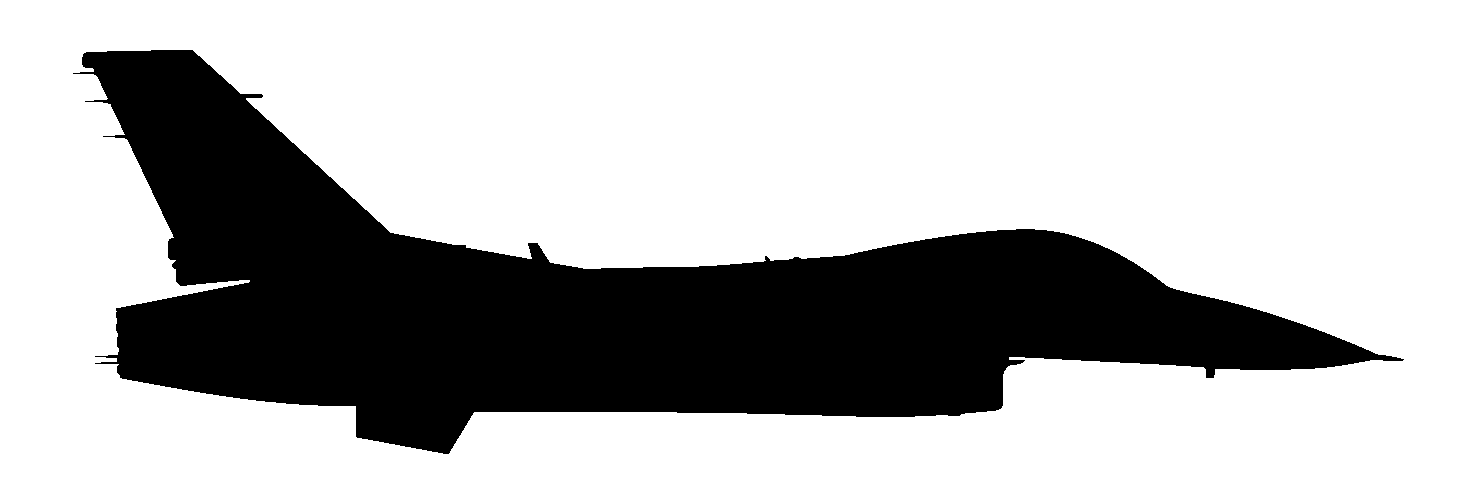
\includegraphics[
                width=7.5mm,
            ]{diagrams/aircraft/silhouette_f16_side.pdf}
        };

        \draw[thin]
        (straightin_a) -- (high_key) -- (30,20)
        (-80,0) -- (td_des);
            
        \draw[->]
        (straightin_a) -- (straightin_base) -- (final) -- (td_des)
        (straightin_b) -- (straightin_base) -- (final) -- (td_des);

        \draw[thin, dashed]
        (straightin_b1) -- (td_des) node[font=\footnotesize, pos=0, above] {11$^\circ$}
        (straightin_b2) -- (td_des) node[font=\footnotesize, pos=0, above] {17$^\circ$}
        (straightin_a) -- (td_des)node[font=\footnotesize, pos=0.10, below] {8$^\circ$};

        \draw[<->, thin]
        (24,20) -- ++(0,-20) node[font=\small, pos=1, below] {7'000 ft};

        \draw[thin]
        (straightin_a) -- ++(0,-20) node[font=\small, pos=1, below] {8 nm}
        (straightin_b1) -- ++(0,-20) node[font=\small, pos=1, below] {6 nm}
        (straightin_b2) -- ++(0,-20) node[font=\small, pos=1, below] {4 nm};
        
        \draw[thin]
        let \p1=(straightin_base) in 
        (straightin_base) -- (10,\y1);
        \draw[<->, thin]
        let \p1=(straightin_base) in 
        (3, \y1) -- (3,0) node[font=\small, pos=1, below] {2'000 ft};

        \node[red, font=\small\bfseries, above] at (straightin_a) {A};
        \node[red, font=\small\bfseries, above] at (straightin_b) {B};
        \filldraw[red] (straightin_a) circle (2pt);
        \filldraw[red] (straightin_b) circle (2pt);
        \filldraw[red] (td_des) circle (2pt);
        \path (-40,20) -- (high_key) node[red, font=\small\bfseries, pos=0.5, above] {C};

        \node[red, font=\footnotesize\bfseries, above, align=left, anchor=south west] at (high_key) {Overhead \\ Approach};
        \filldraw[red] (high_key) circle (2pt);

    \end{tikzpicture}
    \caption{Flameout landing pattern --- straight-in approach}
    \label{fig:proc_em:landing:flameout:straightin}
\end{figure}

% \begin{table}[htbp]
%     \centering
%     \small
%     \caption{Straight-in approach parameters}
%     \begin{tabular}{l r r r r}
%         \toprule
%         \textbf{Point} & \textbf{Range} & \textbf{Angle} & \textbf{AGL} & \textbf{EPU} \\
%         \midrule
%         A & 8 nm & 8$^\circ$ & 7'000 ft & > 45\% \\
%         B & 4 nm & 11-17$^\circ$ & 4-8'000 ft & > 20\% \\
%         C & < 4 nm & > 17$^\circ$ & --- & --- \\
%         \bottomrule
%     \end{tabular}
% \end{table}

\marginfigeometry

\subsubsection{PROCEDURE}

\begin{checklistenumerate}[start=0]
    \blueitem[Select Approach]

    Turn towards suitable runway, 
    accomplish overhead or straight-in approach
    \begin{itemize}
        \item Overhead approach altitudes
        \begin{itemize}
            \item \textbf{High Key --- 7'000-10'000 ft AGL} \\
            7'000 ft plus 500 ft per 1000 lbs of fuel / stores
            \item \textbf{Low Key --- 3'000-5'000 ft AGL}\\
            3'000 ft plus 250 ft per 1000 lbs of fuel / stores
        \end{itemize}
        \item Straight-in approach altitudes
        \begin{itemize}
            \item \textbf{8 nm --- 7'000 ft AGL}\\
            for optimal LG up glideslope until 2'000 ft AGL
            \item \textbf{4 nm --- 4'000-8'000 ft AGL}\\
            Lower LG once desired touchdown point 11-17$^\circ$ below horizon
        \end{itemize}
    \end{itemize}
    \blueitem[Stores]\dotfill \textbf{Jettison}\\
    \hfill(if required)
    \blueitem[Airspeed]\dotfill 200 kts
    \begin{itemize}
        \item increase airspeed 5 kts for every 1000 lbs of fuel / stores
    \end{itemize}
    \blueitem[EPU Switch]\dotfill \textbf{ON}
    \blueitem[JFS Switch]\dotfill \textbf{START 2}\\
    \hfill(below 20'000 ft MSL, 400 kts)
    \blueitem[AIR SOURCE Knob]\dotfill \textbf{RAM}\\
    \hfill(below 25'000 ft MSL)
    \blueitem[LG Handle]\dotfill \textbf{DN}
    \blueitem[ALT GEAR Handle]\dotfill Pull\\
    \hfill(if required)
    \blueitem[Airspeed]\dotfill 190 kts in pattern
\end{checklistenumerate}
\textbf{After Touchdown}
\begin{checklistenumerate}[resume]
    \blueitem[DRAG CHUTE Switch]\dotfill \textbf{DEPLOY}\\
    \hfill(if required)
    \blueitem[HOOK Switch]\dotfill \textbf{DN}\\
    \hfill(if required)
\end{checklistenumerate}

\clearpage

\marginfigrestore